\question{Wellenreflektion} 


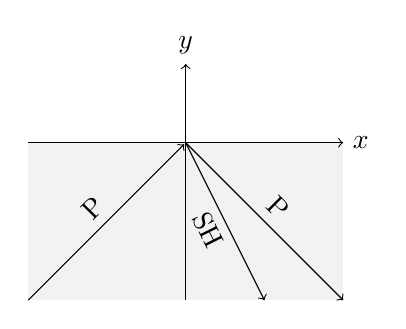
\begin{tikzpicture}
 \fill[black!5!white] (-2,0) rectangle (2,-2);
 \draw[->] (-2,0 ) -- (2,0) node[right] {$x$};
 \draw[->] ( 0,-2 ) -- (0,1) node[above] {$y$};
 \draw[->] (-2,-2) -- node[above, sloped] {P} (-0.02,-0.02);
 \draw[->] (0,0) -- node[below, sloped] {SH} (1, -2);
 \draw[->] (0,0) -- node[above, sloped] {P} (2, -2);
\end{tikzpicture}


In einem linear elastischen, isotropen Kontinuum Elastizitätsmodul $E$ und Querkontraktionszahl $\nu$ trifft eine ebene P-Welle
\begin{equation*}
    \mathbf{u}_1(\mathbf{r},t)=\mathbf{n}_1 A_1 \cos\bigl(\kappa_1 (\mathbf{n}_1\cdot \mathbf{r}-c_\mathrm{P}t)\bigr) 
    \quad \text{mit} \quad
    \mathbf{u}={[u_1,v_1,w_1]}^\mathrm{T}
    \quad \text{und} \quad
    \mathbf{r}={[x,y,z]}^\mathrm{T}
\end{equation*}
auf einen freien Rand. Die entsprechende Randbedingung lautet
\begin{equation*}
    \sigma_{xy}(\mathbf{r}_\mathrm{R},t) = \sigma_{yy}(\mathbf{r}_\mathrm{R},t) = 0
    \quad \text{mit} \quad
    \mathbf{r}_\mathrm{R}={ [x,0,z] }^\mathrm{T}. 
\end{equation*}
Die Ausbreitungsrichtung $\mathbf{n}_1=[\sin\alpha_1, \cos\alpha_1, 0]^\mathrm{T}$, Amplitude $A_1$ und Wellenzahl $\kappa_1$ der einfallenden Welle sind vorgegeben.
Gesucht sind die Darstellungen der reflektierten Wellen
\begin{align*}
    \mathbf{u}_2(\mathbf{r},t) &= \mathbf{n}_2 A_2 \cos\bigl(\kappa_2 (\mathbf{n}_2\cdot \mathbf{r}-c_\mathrm{P}t)\bigr)
    \quad \text{mit} \quad
    \mathbf{n}_2=[\sin\alpha_2,\, -\cos\alpha_2,\, 0]^\mathrm{T}, \\
    \mathbf{u}_3(\mathbf{r},t) &= \mathbf{e}_z\times\mathbf{n}_3 A_3 \cos\bigl(\kappa_3 (\mathbf{n}_3\cdot \mathbf{r}-c_\mathrm{S}t)\bigr)
    \quad \text{mit} \quad 
    \mathbf{n}_3=[\sin\beta,\, -\cos\beta,\, 0]^\mathrm{T} \\
    &\text{und} \quad
    \mathbf{e}_z={[0,0,1]}^\mathrm{T}.
\end{align*}


\begin{minipage}[t]{\linewidth}
    geg.:
    \begin{tasks}
        \task[] elastisches Kontinuum:
        \task[] $\Lambda = \frac{E v}{(1-2v)(1+v)}$ \qquad $\mu = \frac{E}{2(1+v)}$ 
        \task[] einfallende P-Welle:
        \task[] $w_1 = A_1 n_1 \exp(i \ \kappa_1(n_1 r-c_p t))$ \qquad \text{mit:} $n_1 = 
                \begin{bmatrix}
                    \sin(\alpha_1) \\
                    \cos(\alpha_1) \\
                    0
                \end{bmatrix}$ und $r = \begin{bmatrix}
                    x \\ y \\ 0
                \end{bmatrix}$
        \task[] spannungsfreier Rand $y = 0$:
        \task[] $\sigma_{xy} (x,0,z,t) = \sigma_{yy} (x,0,z,t) = 0$
    \end{tasks}
\end{minipage}
\quad
\begin{minipage}[t]{\linewidth}
    ges.:
    \begin{tasks}
        \task[] Randspannungen $\sigma_{xy}$ und $\sigma_{yy}$
        \task[] Amplituden der reflektierten Wellen $A_{P_{ref}}$ und $A_{S_{ref}}$
    \end{tasks}
\end{minipage}

\begin{solution}
    Phasen der einfallenden P-Welle $P_{in}$, der reflektierten P-Welle $P_{ref}$ und der reflektierten SH-Welle $S_{ref}$:
    \begin{align*}
            &\phi_{P_{in}} = \textit{i} \cdot \kappa_P (x \sin(\alpha) + y \cos(\alpha) - c_P t) \\
            &\phi_{P_{ref}} = \textit{i} \cdot \kappa_P (x \sin(\alpha) - y \cos(\alpha) - c_P t) \\
            &\phi_{S_{ref}} = \textit{i} \cdot \kappa_S (x \sin(\beta) - y \cos(\beta) - c_S t)
    \end{align*}

    komplexe Darstellung der Wellenausbreitung aller drei Wellen:

    \begin{align*}
        &P_{in_{complex}} = \hat{A}_{P_{in}} \exp(\phi_{P_{in}}) \\
        &P_{ref_{complex}} = \hat{A}_{P_{ref}} \exp(\phi_{P_{ref}}) \\
        &S_{ref_{complex}} = \hat{A}_{S_{ref}} \exp(\phi_{S_{ref}})
    \end{align*}

    Verschiebungen in Richtung (x,y):

    \begin{align*}
        &x_{P_{in}} = P_{in_{complex}} \sin(\alpha) \\
        &x_{P_{ref}} = P_{ref_{complexx}} \sin(\alpha) \\
        &x_{S_{ref}} = S_{ref_{complex}} \cos(\beta) \\
        \\
        &y_{P_{in}} = P_{in_{complex}} \cos(\alpha) \\
        &y_{P_{ref}} = - P_{ref_{complex}} \cos(\alpha) \\
        &y_{S_{ref}} = S_{ref_{complex}} \sin(\alpha)
    \end{align*}

    Spannungen $\sigma_{xy}$ und $\sigma_{yy}$, die relevant für die Reflexion sind:

    \begin{align*}
        &\sigma_{xy_{Pin}} = \mu (\frac{\delta x_{P_{in}}}{\delta y} + \frac{\delta y_{P_{in}}}{\delta x}) \\
        &\sigma_{xy_{Pref}} = \mu (\frac{\delta x_{P_{ref}}}{\delta y} + \frac{\delta y_{P_{ref}}}{\delta x}) \\
        &\sigma_{xy_{Sref}} = \mu (\frac{\delta x_{S_{ref}}}{\delta y} + \frac{\delta y_{S_{ref}}}{\delta x}) \\
        \\
        &\sigma_{yy_{Pin}} = (2\mu + \Lambda) \frac{\delta y_{P_{in}}}{\delta y} + \Lambda \frac{\delta x_{P_{in}}}{\delta x} \\
        &\sigma_{yy_{Pref}} = (2\mu + \Lambda) \frac{\delta y_{P_{ref}}}{\delta y} + \Lambda \frac{\delta x_{P_{ref}}}{\delta x} \\
        &\sigma_{yy_{Sref}} = (2\mu + \Lambda) \frac{\delta y_{S_{ref}}}{\delta y} + \Lambda \frac{\delta x_{S_{ref}}}{\delta x} \\
    \end{align*}

    Auswertungen der Spannungen am Rand:

    \begin{align*}
        \sigma_{xy_{Rand}} &= \frac{\sigma_{xy_{Pin}} \exp(-\phi_{P_{in}})}{i} + \frac{\sigma_{xy_{Pref}} \exp(-\phi_{P_{ref}})}{i}
                            + \frac{\sigma_{xy_{Sref}} \exp(-\phi_{S_{ref}})}{i} \\
                           &= \mu (\hat{A}_{P_{in}} \kappa_P \sin(2\alpha) - \hat{A}_{P_{ref}} \kappa_P \sin(2 \alpha) 
                            - \hat{A}_{S_{ref}} \kappa_S \cos(2\beta))\\
        \sigma_{yy_{Rand}} &= \frac{\sigma_{yy_{Pin}} \exp(-\phi_{P_{in}})}{i} + \frac{\sigma_{yy_{Pref}} \exp(-\phi_{P_{ref}})}{i}
                            + \frac{\sigma_{yy_{Sref}} \exp(-\phi_{S_{ref}})}{i} \\
                           &= \hat{A}_{P_{in}} \kappa_P (\Lambda + 2 \mu \cos[2](\alpha)) + \hat{A}_{P_{ref}} \kappa_P (\Lambda + 2 \mu \cos[2](\alpha))
                            - \hat{A}_{S_{ref}} \kappa_S \mu \sin(2\beta)
    \end{align*}

    Die Amplituden der reflektierten Wellen sind beide winkelabhängig. Um diese zu berechnen, löst man nun die Randbedingungen nach 
    $A_{P_{ref}}$ und $ A_{S_{ref}}$ auf. Das Ergebnis lautet, wie folgt:

    \begin{align*}
        &A_{P_{ref}} = \frac{
            A_{P_{in}} (- \Lambda \cos(2 \beta) + \mu \sin(2\alpha)\sin(2\beta) - 2 \mu \cos[2](\alpha) \cos(2\beta))
        }{
            \Lambda \cos(2 \beta) + \mu \sin(2 \alpha) \sin(2\beta) + 2 \mu \cos[2](\alpha) \cos(2 \beta)
        } \\
        \\
        &A_{S_{ref}} = \frac{
            2 A_{P_{in}} \kappa_P (\Lambda \sin(2 \alpha) + \mu \sin(2 \alpha) + \frac{\mu \sin(4 \alpha)}{2})
        }{
            \kappa_S (\Lambda \cos(2 \beta) + \mu \cos(2 \beta) + \mu \cos(2\alpha - 2\beta) )
        }\\
    \end{align*}
\end{solution}